\documentclass[
    12pt,               % tamanho da fonte
    openright,         
    oneside,
    a4paper, 
    english,            % idioma adicional para hifenização
    brazil              % o último idioma é o principal do documento
    ]{ifsp-spo-inf-ctds}

\titulo{PETINDER}

\renewcommand{\imprimirautor}{
\begin{tabular}{lr}
BRENDA OLIVEIRA DE SOUSA  & SP1851551 \\
CECÍLIA DUARTE GAMA & SP1852639 \\
EDUARDA BOMFIM DA CONCEIÇÃO & SP1852281 \\
FERNANDA APARECIDA FIGUEIREDO DA SILVA & SP1852124 \\
GABRIELA GONÇALVES MENDONÇA LINO & SP1850814 \\
GIOVANA PAZ PEDROZO & SP185089X \\
\end{tabular}
}

\tipotrabalho{Projeto da Disciplina Prática de Desenvolvimento de Sistemas}

\disciplina{PDS - Prática de Desenvolvimento de Sistemas}

\preambulo{Proposta de projeto para disciplina Prática de Desenvolvimento de Sistemas.}

\data{09 DE JUNHO DE 2021}

\renewcommand{\orientadorname}{Professor:}
\orientador{IVAN FRANCOLIN MARTINEZ}
\renewcommand{\coorientadorname}{Professor:}
\coorientador{LEONARDO ANDRADE MOTTA DE LIMA}


% informações do PDF
\makeatletter
\hypersetup{
        %pagebackref=true,
        pdftitle={\@title}, 
        pdfauthor={\@author},
        pdfsubject={\imprimirpreambulo},
        pdfcreator={LaTeX with abnTeX2},
        pdfkeywords={abnt}{latex}{abntex}{abntex2}{trabalho acadêmico}, 
        colorlinks=true,            % false: boxed links; true: colored links
        linkcolor=blue,             % color of internal links
        citecolor=blue,             % color of links to bibliography
        filecolor=magenta,              % color of file links
        urlcolor=blue,
        bookmarksdepth=4
}
\makeatother


% ----
% Início do documento
% ----
\begin{document}

% Retira espaço extra obsoleto entre as frases
\frenchspacing 

\pretextual

\imprimircapa

\imprimirfolhaderosto

\pdfbookmark[0]{\listfigurename}{lof}
\listoffigures*
\cleardoublepage
% ---

\pdfbookmark[0]{\listofquadrosname}{loq}
\listofquadros*
\cleardoublepage

\pdfbookmark[0]{\contentsname}{toc}
\tableofcontents*
\cleardoublepage

% ----------------------------------------------------------
% ELEMENTOS TEXTUAIS
% ----------------------------------------------------------
\textual

% ----------------------------------------------------------
% Introdução
% ----------------------------------------------------------
\chapter[Introdução]{Introdução}
No Brasil temos muitos casos de abandonos de animais. Em 2019 o Instituto Pet Brasil realizou um levantamento a respeito de animais sob tutela de \ac{ONGs}, e chegaram ao resultado de mais de 170 mil animais. Desses, 96\% são cachorros e apenas 4\% são gatos. Além das \ac{ONGs} muitas pessoas resgatam animais que encontram na rua em situações de vulnerabilidade, levam para suas casas e fornecem lares temporários até encontrarem, então, uma família que possa oferecer todo cuidado que o animal necessita \cite{tutelaONG}.

O ano de 2020 foi marcado pela pandemia da \gls{COVID-19}, devido a isso, a população foi submetida a um período de quarentena obrigatória. Nos primeiros meses, com mais tempo em casa, os brasileiros recorreram a \ac{ONGs} em busca de companhia animal, aumentando os números de adoções \cite{adocao}.

O país foi afetado em diversas questões: econômica, social, política e culturalmente, causando, assim, uma reviravolta na vida de todos, inclusive dos animais. Novamente o índice de abandono cresce, e com alguns fatores como desemprego em grandes níveis, retorno de atividades presenciais, fim do auxílio emergencial, o cuidado dos amimais ficou inviável para alguns tutores \cite{abandono_pandemia}. 

Visando facilitar o processo de adoção, tanto para o adotante, como para o doador, a equipe TI TI TI decidiu por desenvolver um \textit{website} que atendesse às necessidades dos usuários, possibilitando a busca por um animal que combine com as premissas do adotante.

\section{Problema a ser solucionado}
Em 2013 a \ac{OMS} lançou uma nota que continha estimativas do número de animas vivendo nas ruas do Brasil, eram cerca de 20 milhões de cães e 10 milhões de gatos. Em cidades grandes como São Paulo e Rio de Janeiro há um cachorro a cada 5 habitantes, e 10\% destes não tem um lar.

Com o início da pandemia e confinamento brasileiro, as \ac{ONGs} passaram a reportar um aumento na procura de adoção de cães e gatos. Segundo o médico veterinário que é gerente de vigilância do \ac{CCZ} do Distrito Federal, Rodrigo Menna Barreto, o número de adoções de animais registrados pelo órgão entre janeiro e setembro de 2020 foi maior que o dobro registrado em todo o ano anterior.

Infelizmente essa rara notícia boa não durou, quando a pandemia passou a viver seu pior momento no Brasil com crise social e econômica, muitos dos animais voltaram ao seu destino anterior sendo abandonados ou devolvidos por famílias que alegaram falta de condições financeiras ou psicológicas para cria-los, além daqueles que os abandonavam por medo de ter \gls{COVID-19} por transmissão de cães e/ou gatos (uma informação comprovada falsa). Isso levou a \ac{ONGs} superlotadas e recordes de abandono.

\section{Justificativa}
Diariamente ao sairmos de nossas casas, cenas de cães e gatos abandonados são muito comuns, principalmente em centros urbanos, onde reside a maior parte da população. Na pandemia é notável que essas cenas acabaram ficando cada vez mais frequente, tornando a reflexão acerca do tema um tanto relevante.

De acordo com dados da \gls{AMPARA}, cerca de 60\% a 70\% de animais foram abandonados, entre julho de 2020 e fevereiro de 2021 (em comparação com 2019). Um dos muitos motivos para tal estimativa é a dificuldade financeira, e adoção por impulso durante o período de quarentena \cite{abandono}.

Em vista de tais dados, nossa equipe se sensibilizou com a causa e decidiu criar um projeto que realize a adoção de cães e gatos de forma prática e efetiva, contribuindo, dessa forma, com a diminuição dos números de abandonos, de maneira consciente e solidária.

\section{Objetivos}

A equipe TI TI TI desenvolveu o \textit{website} PETINDER visando prover para os usuários da plataforma um local seguro onde possa acontecer a conexão entre animal e adotante. Temos como objetivo também auxiliar na queda dos números de animais em situação de rua e ajudar cães e gatos a encontrarem novos lares onde possam receber proteção e afeto.

O projeto tem como objetivos específicos:

\begin{itemize}
\item Facilitar o processo de adoção de cães e gatos;
\item Oferecer uma plataforma segura e intuitiva para o usuário;
\item Colaborar com a diminuição do número de animais abandonados do país.
\end{itemize}

% ---
% Capitulo de revisão de literatura
% ---
\chapter{Revisão da Literatura}
A revisão da literatura é a etapa do trabalho em que se reúne as fontes de pesquisa que vão fornecer embasamento teórico para o trabalho.

Além disso, serve para dialogar com essas referências e aplicar seus conceitos no tema da monografia.

Portanto, é na revisão da literatura onde deve-se apresentar um levantamento bibliográfico acerca do assunto que será tratado na monografia, com escopo definido e uma análise crítica sobre os autores selecionados. 

%Todos trabalhos devem possuir a revisão de literatura onde são abordados os estudos feitos com base da literatura (livros, artigos acadêmicos, publicações em periódicos), todos elementos devem ser referenciados por citações.

%Não são abordados aqui itens técnicos que normalmente são vistos em disciplinas anteriores do curso (UML, banco de dados, metodologias de gerenciamento de projeto etc...)

\section{Assunto X}

\chapter{Descrição funcional da aplicação}
% Falar das funcionalidades da aplicacao, das partes interessadas, e dos concorrentes (incluir tabela de comparacao)

\section{Casos de uso}
% Descricao e diagrama

\input{desenvolvimento/texto-modelagem}

%----------------------------------------------------------------------
\chapter{Funcionalidades}
Assim como ilustra a \autoref{fig_diag_virado}, o usuário pode acessar o site sem efetuar cadastro ou login. Dessa forma, seu acesso será restrito apenas a timeline (\autoref{fig_timeline}) e aos perfis dos animais (\autoref{fig_perfil}), precisando estar logado em uma conta para acessar outros recursos, como doar e/ou adotar um animal.

% DELIMITAR DISTANCIA -------------------------------------------------
\section{Delimitar distância}
Após realizar o cadastro, o sistema deve pedir a permissão do usuário para acessar sua localização. Dessa forma, será possível encontrar os animais mais próximos a ele e delimitar a exibição por proximidade, evitando problemas de deslocamento em maiores distâncias, que poderiam atrapalhar, ou até mesmo impedir a adoção.
%----------------------------------------------------------------------

% ADOTAR --------------------------------------------------------------
\section{Adotar}
Para adotar um animal, o usuário, já cadastrado, deve preencher um formulário de adoção, como na \autoref{fig_formulario}, informando dados pessoais importantes para o doador do animal. Em seguida, deve realizar a procura de animais que pode ser feita de três maneiras diferentes. São elas: 
\begin{itemize}
\item Manual: o usuário pode procurar pelo animal que mais lhe agradar através da timeline, observando a foto do animal e as informações primárias disponíveis nela;
\item Com filtros: a procura pode ser feita com o auxílio de filtros que produzem resultados delimitados através das preferências do usuário;
\item Combinação perfeita: através desse recurso, o usuário não precisa procurar um animal compatível com suas preferências, o sistema faz isso para ele, comparando algumas das informações dadas por ele no formulário de adoção e as de cada um dos animais informadas no momento do cadastro (\autoref{fig_cad_animal}).
\end{itemize}
%----------------------------------------------------------------------

% MATCH ---------------------------------------------------------------
\section{Match}
Ao encontrar o animal que deseja adotar, o usuário tem a opção de curtir o perfil, o que gera uma notificação para o doador desse respectivo animal, que poderá retribuir a curtida ou não. Caso isso ocorra, acontecerá o match, que colocará os dois usuários (adotante e doador) em contato através do chat do site e mudará o status do animal de "disponível" para "em processo de adoção", impossibilitando outros adotantes de curtirem esse animal.
Enquanto um animal está em processo de adoção, outros usuários ficam impossibilitados de curtir ele, mas, podem entrar em uma fila de espera para match no caso da adoção com o adotante da vez não acontecer.
%----------------------------------------------------------------------

% MONITORAMENTO DE CHAT -----------------------------------------------
\section{Monitorar chat}
Durante o processo de adoção, enquanto os usuários adotante e doador estiverem em contato no chat, as mensagens trocadas serão monitoradas, de forma que, em caso de usarem palavras registradas no sistema como impróprias, o usuário que a enviou terá cometido uma infração. Caso o mesmo usuário cometa três infrações, sua conta será banida temporariamente e, e caso uma mesma conta seja banida três vezes, será excluida permanentemente.
%----------------------------------------------------------------------
\begin{figure}[htb]
    \centering
	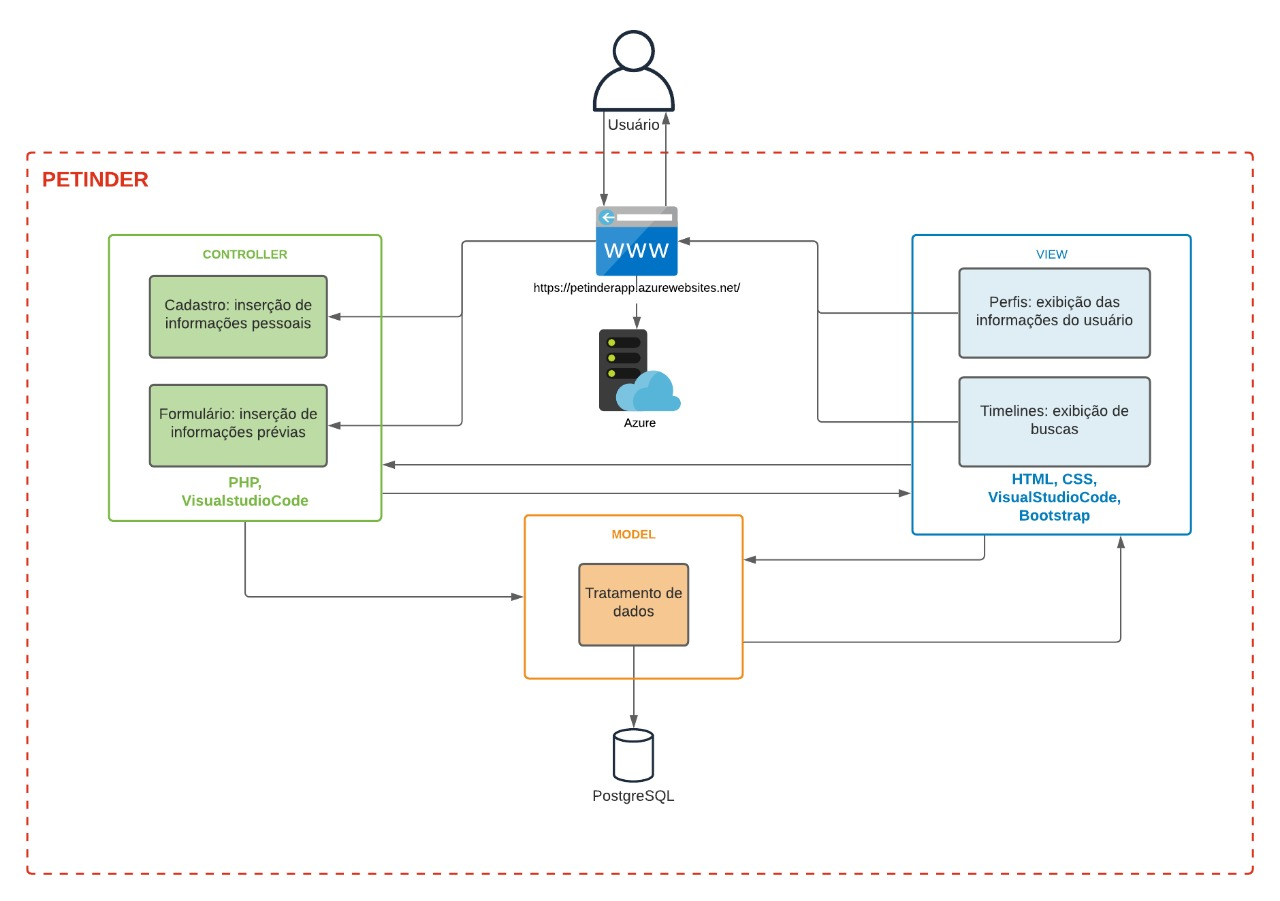
\includegraphics[width=1\textwidth]{imagens/diagrama_de_arquitetura.jpg}
	\caption{\label{fig_diagrama}Diagrama de arquitetura do sistema}
	\fonte{Elaborada pelos autores}
\end{figure}


%--------------------------------------------------------------------------
\chapter{Tecnologias}
As tecnologias que serão utilizadas durante o ano na disciplina, não apenas no desenvolvimento da aplicação, mas também na redação da documentação, e no registro de atividades e entregas, serão:
\begin{itemize}
\item Front-end: HTML5, CSS3 e JavaScript;
\item Framework: Bootstrap 4;
\item Back-end: PHP;
\item Banco de dados: PostgreSQL com a extensão geoespacial PosGIS;
\item IDE: Visual Studio Code e Eclipse;
\item Documentos: \LaTeX;
\item Controle de Versão: Subversion;
\item Gource;
\end{itemize}

%--------------------------------------------------------------------------
\chapter{Equipe}
A equipe TI TI TI é composta por seis integrantes e possui esse nome como uma referência a relação do nome da novela da Rede Globo Ti-Ti-Ti e a sigla da área do conhecimento Tecnologia da Informação (TI), e deve ser lido como uma tripla repetição da sigla. A divisão de tarefas da equipe no desenvolvimento do PETINDER pode ser observada no \autoref{quadro}.

\input{desenvolvimento/quadro}
%--------------------------------------------------------------------------
%--------------------------------------------------------------------------
%----------------------------------------------------------------------

\phantompart
\postextual

\bibliography{referencias.bib,abntex2-doc-abnt-6023.bib}

\end{document}